\section{Regressão Linear}
\label{s.linear_regression}

\subsection{Uma Variável (Univariado)}
\label{ss.one_variable}
 
 Suponha que tenhamos o problema de predizer preços de casas, como demonstradas abaixo. A regressão do problema tem por objetivo estimar (predizer) valores reais de saída, dado uma entrada. Considerando o problema mencionado, gostaríamos de estimar o preço de uma casa dado o seu tamanho, isto é, gostaríamos de encontrar a \textbf{linha reta} a qual melhor se adapta aos pontos da base de dados (dados de treinamento).\\
 
  \begin{center}
 	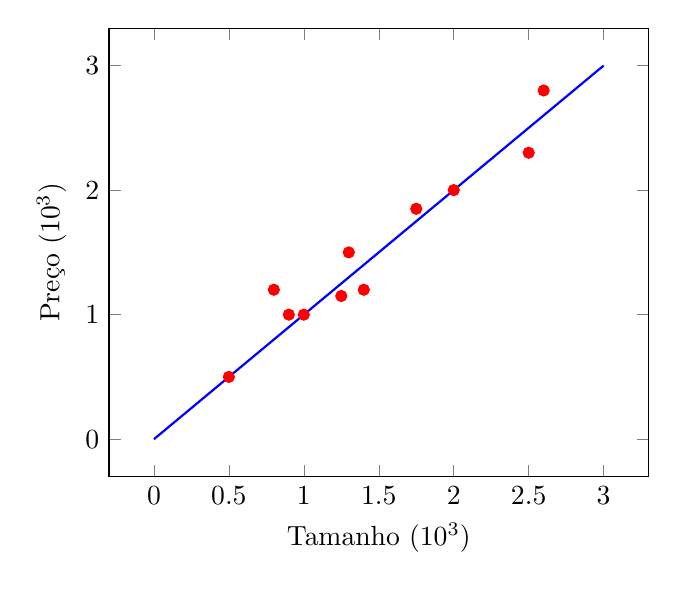
\begin{tikzpicture}[domain=0:3]
  	\begin{axis}[ 
    	xlabel=Tamanho ($10^3$),
    	ylabel={Preço ($10^3$)}
  		] 
    	\addplot[blue, thick] {x}; 
    	\addplot[only marks, red] plot coordinates {
        (0.5,0.5)
        (0.9,1)
        (1, 1)
        (0.8,1.2)
        (1.25, 1.15)
        (1.4, 1.2)
        (1.3, 1.5)
        (1.75, 1.85)
        (2, 2)
        (2.5, 2.3)
        (2.6, 2.8)
        
    };
  	\end{axis}
	\end{tikzpicture}
 \end{center}
 
 \textbf{Exemplo:} Seja $m$ o número de exemplos de treinamento, $x \in \mathbb{R}$ a variável de entrada (características) e $y \in \mathbb{R}$ a variável de saída (objetivo). Então, um treinamento simples de treinamento é denotado por $(x, y)$, sendo o conjunto de treinamento $X$ composto por todas as amostradas de treinamento, isto é, $X = \{(x, y), (x_2, y_2), \dots, (x_m, y_m)\}$. Usualmente, nós possuímos o seguinte fluxo de dados:
 
 \begin{center}
 Dados de treinamento $X \longrightarrow$ Algoritmo de treinamento $\longrightarrow h$ (tamanho da casa) $\longrightarrow$ preço estimado	
 \end{center}

 A função linear pode ser definida como $h_w(x) = w_0 + w_1x$, onde $w_0$ e $w_1$ são os parâmetros do modelo. Suponha que tenhamos os seguintes exemplos:
 
 \begin{center}
 	\begin{tikzpicture}[domain=0:3]
  	\begin{axis}[ 
    	xlabel=$x$,
    	ylabel={$h_w(x) = 1.5 + 0x$}
  		] 
    	\addplot[blue, thick] {1.5 + 0*x}; 
  	\end{axis}
	\end{tikzpicture}
 \end{center}
 
  \begin{center}
 	\begin{tikzpicture}[domain=0:3]
  	\begin{axis}[ 
    	xlabel=$x$,
    	ylabel={$h_w(x) = 0.5x$}
  		] 
    	\addplot[blue, thick] {0.5*x}; 
  	\end{axis}
	\end{tikzpicture}
 \end{center}
 
  \begin{center}
 	\begin{tikzpicture}[domain=0:3]
  	\begin{axis}[ 
    	xlabel=$x$,
    	ylabel={$h_w(x) = 1 + 0.5x$}
  		] 
    	\addplot[blue, thick] {1 + 0.5*x}; 
  	\end{axis}
	\end{tikzpicture}
 \end{center}
 
 Portanto, possuímos diferentes comportamentos envolvendo $h_w(x)$, o qual é chamado de \textbf{função hipótese}. \\
 
 A ideia principal da regressão linear é escolher $w_0$ e $w_1$ tal que $h_w(x)$ esteja o mais próximo de $y$, considerendo os exemplos de treinamento $(x_i, y_i)$, $i = 1, 2, \dots, m$. Para cumprir tal propósito, temos que solucionar o seguinte problema de otimização:
 
 \begin{equation}
 \label{eq.mse}
 minimizar_{w_0, w_1} \quad \frac{1}{2m} \sum_{i=1}^{m} (h_w(x_i) - y_i)^2
 \end{equation}
 
 onde $h_w(x_i)$ é o \textbf{preço estimado} e $y_i$ é o \textbf{preço real}. \\
 
 A Equação~\ref{eq.mse} é usualmente chamada de \textbf{função de custo}, a qual também é conhecida como Erro Médio Quadrático (\emph{Mean Squared Error} - MSE). Podemos simplificar a notação e reescrever a Equação~\ref{eq.mse} como seguinte:
 
 \begin{equation}
 \label{eq:simplify_mse}
minimizar_{w_0, w_1} \quad J(w_0, w_1)	
 \end{equation} \\
 
 onde $J(w_0, w_1) = \frac{1}{2m} \sum_{i=1}^{m} (h_w(x_i) - y_i)^2$. Também podemos simplificar ainda mais considerando que $w_0 = 0$. Portanto, possuíremos as seguintes equações para representar as funções de hipótese e custo, respectivamente:
 
 \begin{equation}
 \label{eq:hip_function}
h_w(x) = w_1x
 \end{equation}

e

 \begin{equation}
 \label{eq:cost_function}
J(w_1) = \frac{1}{2m} \sum_{i=1}^{m} (h_w(x_i) - y_i)^2
 \end{equation} \\
 
  O problema de minimização torna-se agora:
 
 \begin{equation}
 \label{eq:min_problem}
minimizar_{w_1} \quad J(w_1)
 \end{equation} \\
 
 Tentemos entender ambas funções de hipótese e custo.
 
   \begin{center}
 	\begin{tikzpicture}[domain=0:3]
  	\begin{axis}[ 
    	xlabel=$x \mid {w_1 = 1}$,
    	ylabel={$h_w(x) = x$}
  		] 
    	\addplot[red, thick] {x}; 
  	\end{axis}
	\end{tikzpicture}
 \end{center}
 
 \begin{center}
 $J(w_1) = \frac{1}{2m} \sum_{i=1}^{m} (h_w(x_i) - y_i)^2$\\~\\
 $= \frac{1}{2m} \sum_{i=1}^{m} (w_1 x_i) - y_i)^2$\\~\\
 $= \frac{1}{2\times3} [(1-1)^2 + (2-2)^2 + (3-3)^2]$\\~\\
 $= \frac{1}{6} \times 0 = 0$\\~\\
\end{center}

   \begin{center}
 	\begin{tikzpicture}[domain=0:3]
  	\begin{axis}[ 
    	xlabel=$x \mid {w_1 = 0.5}$,
    	ylabel={$h_w(x) = 0.5x$}
  		] 
    	\addplot[red, thick] {0.5*x}; 
  	\end{axis}
	\end{tikzpicture}
 \end{center}
 
  \begin{center}
 $J(w_1) = \frac{1}{2\times3} [(0.5-1)^2 + (1-2)^2 + (1.5-3)^2]$\\~\\
 $= \frac{1}{6} \times (0.25 + 1+ 2.25) \approx 0.58$\\~\\
\end{center}

Se continuarmos efetuando os cálculos mencionados acima para diversos valores de $w_1$, devemos ter algo similar ao seguinte gráfico:\\~\\

  \begin{center}
 	\begin{tikzpicture}[domain=-3:3]
  	\begin{axis}[ 
    	xlabel=$w_1$,
    	ylabel={$J(w_1)$}
  		] 
    	\addplot[blue, thick] {x^2}; 
  	\end{axis}
	\end{tikzpicture}
 \end{center}
 
 \textbf{Erro Médio Absoluto:}
 \begin{center}
$J(w_1) = \frac{1}{m} \sum_{i=1}^{m} (h_w(x_i) - y_i)$\\~\\
 \end{center}
 
 Portanto, $w_1 = 1$ é o valor o qual minimiza $J(w_1)$ para o exemplo acima. Porque é melhor empregar o MSE ao invés do Erro Médio Absoluto (\emph{Mean Absolute Error} - MAE)? Dado que os erros estão sendo elevados ao quadrado logo após serem ponderados, o MSE resulta em um peso maior relativo à erros maiores. \\
 
 Então, a questão agora é: como podemos encontrar valores plausíveis para ambos $w_0$ e $w_1$? Podemos modelar tal problema como uma tarefa de otimização utilizando o algoritmo do \textbf{Gradiente Descendente} (\emph{Gradient Descent} - GD) por exemplo. Em resumo, temos o seguinte:
 
 \begin{center}
Temos alguma função $J(w_0, w_1)$;\\
Queremos minimizar $J(w_0, w_1)$.\\~\\
 \end{center}
 
 \textbf{Algoritmo do Gradiente Descendente:}
 
 \begin{itemize}
 \item comece com algum $w_0,w_1$;
 \item continue mudando $w_0,w_1$ de modo que reduza $J(w_0,w_1)$ até que atinja o mínimo (\textcolor{red}{isso pode não acontecer!}).\\	
 \end{itemize}
 
 Observemos o mecanismo de busca do Gradiente Descendente:
 
   \begin{center}
 	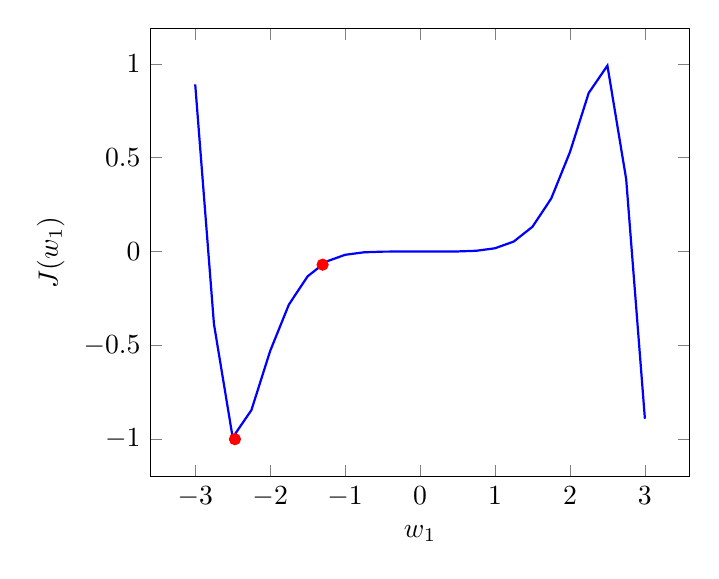
\begin{tikzpicture}[domain=-3:3]
  	\begin{axis}[ 
    	xlabel=$w_1$,
    	ylabel={$J(w_1)$}
  		] 
    	\addplot[blue, thick] {sin(x^5)};
    	\addplot[only marks, red] plot coordinates {
        (-2.47, -1)
        (-1.3, -0.07)};
  	\end{axis}
	\end{tikzpicture}
 \end{center}
 
 A ideia acima pode ser matematicamente formulada como seguinte:
 
 \begin{equation}
 \label{eq:gd}
 w_j = w_j - \alpha \frac{\partial J(w_0,w_1)}{\partial w_j}, j \in \{0, 1\}
 \end{equation} \\
 
 onde $\alpha$ é a taxa de aprendizado e $\frac{\partial J(w_0,w_1)}{\partial w_j}$ é o termo derivativo. \\
 
 A equação acima é chamada de \textbf{regra de atualização}. Segue abaixo a implementação correta desse procedimento:
 
 \begin{center}
 $tmpw_0 = w_0 - \alpha \frac{\partial J(w_0,w_1)}{\partial w_0}$ \\
 $tmpw_1 = w_1 - \alpha \frac{\partial J(w_0,w_1)}{\partial w_1}$ \\
 $w_0 = tmpw_0$ \\
 $w_1 = tmpw_1$ \\~\\
 \end{center}
 
 A próxima questão que pode surgir é como computar o termo derivativo? Suponha que tenhamos apenas um parâmetro, por exemplo, $w_1$. Então, queremos minimizar $J(w_1)$ para algum $w_1 \in \mathbb(R)$. Conhecemos o formato de $J(w_1)$:
 
   \begin{center}
 	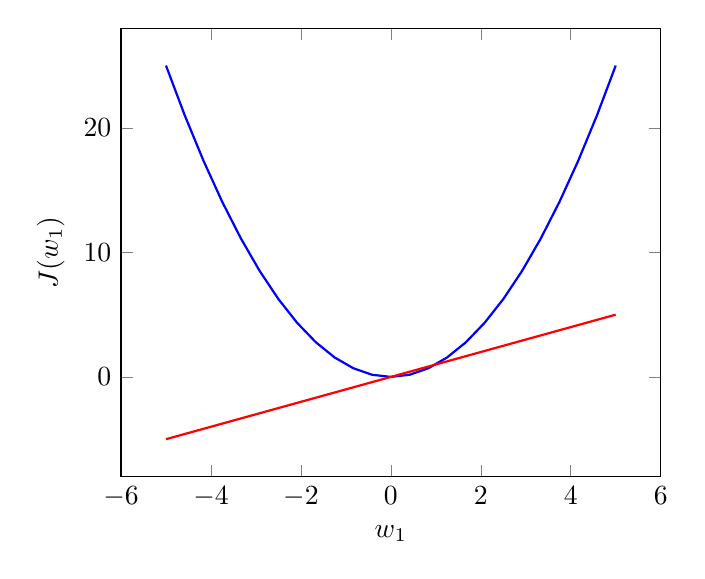
\begin{tikzpicture}
  	\begin{axis}[ 
    	xlabel=$w_1$,
    	ylabel={$J(w_1)$}
  		] 
    	\addplot[blue, thick] {x^2}; 
    	\addplot[red, thick] {x}; 
  	\end{axis}
	\end{tikzpicture}
 \end{center}
 
 onde a linha vermelha é a tangente e a inclinação = $w_1^{t+1} = w_1^t - \alpha \frac{\partial J(w_1)}{\partial w_1} > 0$. \\

O que é uma derivada em um ponto dado? É a \textbf{inclinação} da reta tangente em respeito ao ponto em questão. A inclinação nos indica o ângulo de uma reta em relação à linha horizontal. \\

   \begin{center}
 	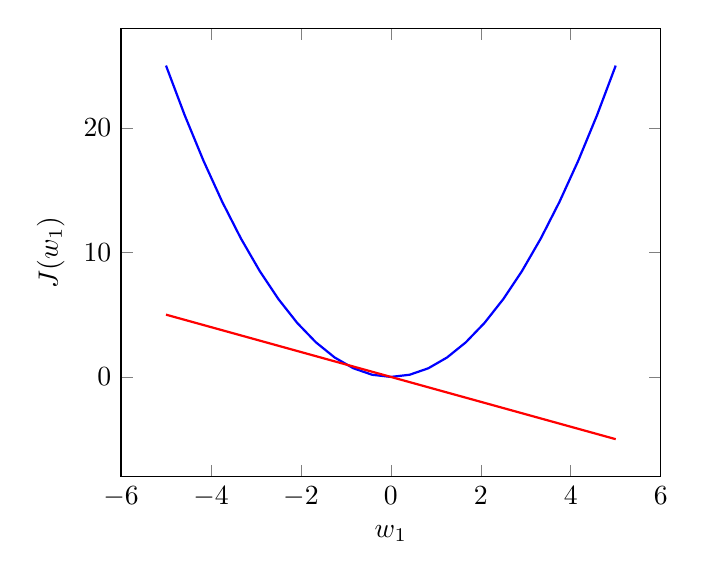
\begin{tikzpicture}
  	\begin{axis}[ 
    	xlabel=$w_1$,
    	ylabel={$J(w_1)$}
  		] 
    	\addplot[blue, thick] {x^2}; 
    	\addplot[red, thick] {-x}; 
  	\end{axis}
	\end{tikzpicture}
 \end{center}
 
 onde a inclinação é igual a $w_1^{t+1} = w_1^t - \alpha \frac{\partial J(w_1)}{\partial w_1} < 0$. \\

Agora, qual é a importância da taxa de aprendizado? Basicamente, pequenos valores de $\alpha$ tendem à uma lenta taxa de convergência, enquanto valores altos de $\alpha$ nos leva à altas taxas de convergência. \\

O que acontece se inicializarmos o GD em um mínimo local?

   \begin{center}
 	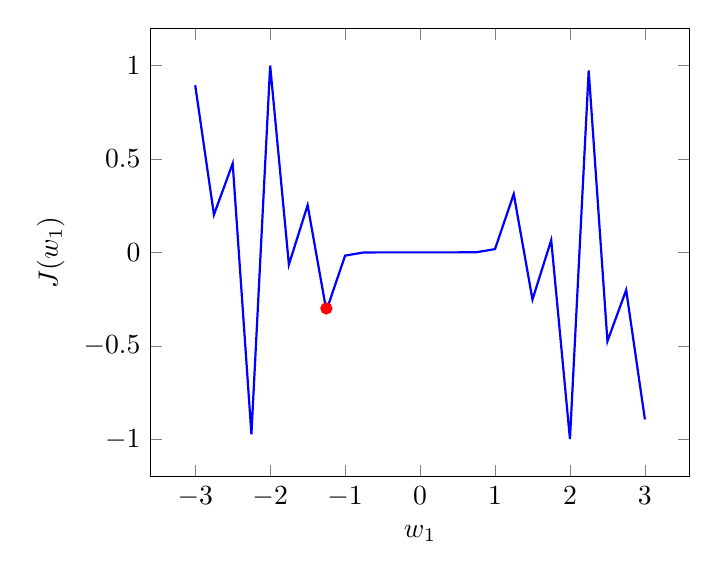
\begin{tikzpicture}[domain=-3:3]
  	\begin{axis}[ 
    	xlabel=$w_1$,
    	ylabel={$J(w_1)$}
  		] 
    	\addplot[blue, thick] {sin(x^13)};
    	\addplot[only marks, red] plot coordinates {
        (-1.25, -0.30)};
  	\end{axis}
	\end{tikzpicture}
 \end{center}
 
 Assim que nos aproximamos do mínimo global / local, o GD leva em consideração passos menores, até mesmo para um $\alpha$ fixo, dado que a inclinação também utiliza valores menores. \\
 
 As derivadas parciais são computadas como seguinte:
 
 \begin{center}
 $\frac{\partial J(w_0, w_1)}{\partial w_0} = \frac{1}{m} \sum_{i=1}^{m}(h_w(x_i) - y_i)$ \\~\\
 
  $\frac{\partial J(w_0, w_1)}{\partial w_0} = \frac{1}{m} \sum_{i=1}^{m}[(h_w(x_i) - y_i)x_i]$ \\
 \end{center}
 
 Portanto, podemos sumarizar o algoritmo do GD como segue: \\
 
 repita até convergência \{ \\ \\
 \hspace*{25pt} $w_0 \leftarrow w_0 - \alpha \frac{1}{m} \sum_{i=1}^{m}(h_w(x_i) - y_i)$ \\~\\
 \hspace*{25pt} $w_1 \leftarrow w_1 - \alpha \frac{1}{m} \sum_{i=1}^{m}[(h_w(x_i) - y_i)x_i]$ \\ \\
 \hspace*{15pt} \}
 
\subsection{Múltiplas Variáveis (Multivariado)}
\label{ss.multi_variables}

Suponha que tenhamos múltiplas características para representar o problema de estimar o preço de uma casa, por exemplo, o número de quartos, o número de andares, dentre outros. Seja $n$ o número de características, tal que nossa função de hipótese possa ser denotada como segue:

\begin{equation}
\label{e.multi_optimization}
h_w(x) = w_0 + w_1x_1 + w_2x_2 + \dots + w_nx_n
= w_0 + \sum\limits_{i = 1}^n w_ix_i.
\end{equation}

Neste caso, temos que $x_i \in \mathbb{R}$. Para a conveniência da notação, seja $x_0 = 1$, tal que $x = [x_0, x_1, x_2, \dots, x_n] \in \mathbb{R}^{n+1}$, e $w = [w_0, w_1, w_2, \dots, w_n] \in \mathbb{R}^{n+1}$. Portanto, a Equação~\ref{e.multi_optimization} pode ser reescrita como segue:

\begin{equation}
\label{e.multi_optimization2}
h_w(x) = w_0x_0 + \sum\limits_{i = 1}^n w_ix_i = \sum\limits_{i = 0}^n w_ix_i = wx^T.
\end{equation}

Então, como podemos utilizar o Gradiente Descendente para a regressão linear multivariável? Agora temos as seguintes proposições:

\begin{center}
função de hipóstese: $h_w(x) = wx^T$\\
função de custo: $J(w) = \frac{1}{2m} \sum\limits_{i=1}^m (h_w(x_i)-y_n)^2$\\
parâmetro: w	
\end{center}

\textbf{Gradiente Descendente:}

 repita até convergência \{ \\ \\
 \hspace*{25pt} $w_j \leftarrow w_j - \alpha \frac{\partial J(w)}{\partial w_j}$\\~\\
 \hspace*{25pt} \textcolor{red}{não esqueça de atualizar cada $w_j$ simultaneamente:}\\~\\
 \hspace*{25pt} $\partial w_j = \frac{1}{m} \sum_{i=1}^{m}[(h_w(x_i) - y_i)x_i^j] \mid j = 1, 2, \dots, n.$ \\ \\
 \hspace*{15pt} \} \\
 
Para trabalharmos com o Gradiente Descendente, podemos utilizar alguns artifícios. Um deles é o \textbf{dimensionamento das características}, i.e. temos que ter certeza de que as características estão em escalas similares.\\

\textbf{Exemplo 1:}

$x_1 =$ tamanho($0 - 200$ feet)$^2$ e $x_2 =$ \# de quartos. \\

\textbf{Exemplo 2:}

$x_1' = \frac{tamanho}{2000}$ e $x_2' = \frac{\# de quartos}{5}$. \\

Portanto, podemos ter cada característica no intervalo aproximado de $-1 \leq x_i^j \leq 1$. Outra maneira é utilizar a \textbf{normalização média}:

\begin{equation}
\label{e.mean_normalization}
x_i^j = \frac{x_i^j - \mu^j}{\beta_{max}^j - \beta_{min}^j},	
\end{equation}

onde $\mu^j$ é o valor médio da característica $j$ no conjunto de treinamento, e $\beta_{max}^j$ e $\beta_{min}^j$ denota os valores máximos e mínimo de cada características $j$ no conjunto de treinamento, $i = 1, 2, \dots, m$ e $j = 1, 2, \dots, n$. Portanto, a ideia é fazer com que as características possuam aproximadamente média igual a zero.

Outro artifício para o Gradiente Descendente é a otimização da taxa de treinamento $\alpha$. Entretanto, previamente, é necessário ter certeza de que o Gradiente Descendente está funcionando corretamente. Um comportamento esperado pode ser ilustrado como segue:

   \begin{center}
 	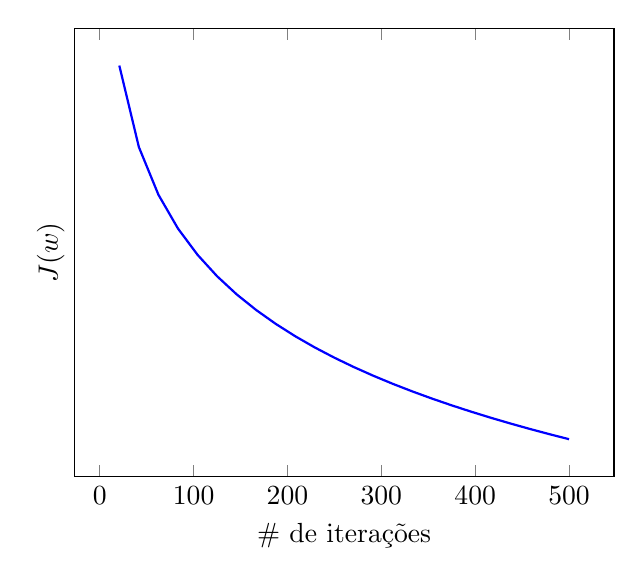
\begin{tikzpicture}[domain=0:500]
  	\begin{axis}[ 
    	xlabel=\# de iterações,
    	ylabel={$J(w)$},
    	ytick=\empty
  		] 
    	\addplot[blue, thick] {-ln(x)};
  	\end{axis}
	\end{tikzpicture}
 \end{center}

\textbf{Problema:} \textcolor{red}{o número de iterações usualmente varia para cada problema. Portanto, é possível parar o algoritmo do GD utilizando a seguinte regra:}

\begin{equation}
\mid J(w)^{t+1} - J(w)^t \mid < \epsilon,
\end{equation}
 
 onde $J(w)^t$ é o valor de cada função de custo na iteração $i$, e $\epsilon$ denota uma quantia muito pequena do \textbf{erro desejado} (usualmente $\epsilon = 10^{-3}$).
 
 Entretanto, se valores de $J(w)$ estão crescendo, é possível utilizar valores menores para $\alpha$. Situações possíveis:
 
    \begin{center}
 	\begin{tikzpicture}[domain=0:10]
  	\begin{axis}[ 
    	xlabel=\# de iterações,
    	ylabel={$J(w)$},
    	xtick=\empty,
    	ytick=\empty
  		] 
    	\addplot[blue, thick] {2^x};
  	\end{axis}
	\end{tikzpicture}
 \end{center}
 
\begin{figure}[h]
\hspace*{66pt}
\includegraphics[scale=0.63]{figs/gd_multi_graph.png}
\label{f.gd_multi_graph}
\end{figure}

\subsection{Ferramentas Adicionais}
\label{s.additional_tools}

No caso de possuirmos espaços de características complexos, pode ser necessário empregar funções de regressão diferentes. Podemos utilizar, por exemplo, polinômios de grau 2:

\begin{equation}
\label{e.second_regression}
h_w(x) = w_0x_0 + w_1x_1 + w_2x^2.	
\end{equation}

Adicionalmente, é provável que os preços das casas comecem a estabilizar depois de um certo tamanho.

Considerando a regressão linear multivariável, ao invés de computar derivadas parciais para posterior computação do Gradiente Descendente, podemos resolver analiticamente a Equação~\ref{e.multi_optimization2}. Basicamente, podemos reescrever a Equação~\ref{e.multi_optimization2} como segue:

\begin{equation}
\label{e.multi_optimization3}
y_i = w^Tx_i, \forall i = 1, 2, \dots, m.
\end{equation}

Seja $X$ a matriz contendo todas as amostras de treinamentos, por exemplo:

\[X=
  \begin{bmatrix}
    x_1^0 & x_1^1 & x_1^2 & \dots & x_1^n \\
    x_2^0 & x_2^1 & x_2^2 & \dots & x_2^n \\
    \vdots & \ddots & & & \vdots \\
    x_m^0 & x_m^1 & x_m^2 & \dots & x_m^n \\
  \end{bmatrix}, \in \mathbb{R}^{m\times (n+1)}\] \\

Adicionalmente, seja $Y$ a matriz contendo todos os preços reais, por exemplo: 

\[Y=
  \begin{bmatrix}
    y_1 \\
    y_2 \\
    \vdots \\
    y_m
  \end{bmatrix}, \in \mathbb{R}^{m\times1}\] \\
  
Podemos reescrever a Equação~\ref{e.multi_optimization3} considerando todos os pontos dos dados de treinamento como segue:
  
\begin{equation}
\label{e.linear_system}
Y = w^TX.	
\end{equation}

Como podemos observar, a equação acima modela um sistema linear, que pode ser solucionado como segue:

\begin{equation}
\label{e.solution_linear_system}
w = (X^TX)^{-1}X^TY,
\end{equation}

onde $A^{-1}$ é o inverso da matriz $A = X^TX$. Em suma, podemos sumarizar os seguintes pontos para cada técnica:

\begin{itemize}
\item \textbf{Gradiente Descendente:} necessita da escolha de $alpha$, necessita várias iterações, funciona muito bem até para $n \rightarrow \infty$;
\item \textbf{Equação:} não necessita da escolha de $\alpha$, não necessita iterar, necessita computar $(X^TX)^{-1}$, o qual pode ser lento quando $n \rightarrow \infty$.
\end{itemize} 